\documentclass[a4paper]{book}
\usepackage{makeidx}
\usepackage{natbib}
\usepackage{graphicx}
\usepackage{multicol}
\usepackage{float}
\usepackage{listings}
\usepackage{color}
\usepackage{ifthen}
\usepackage[table]{xcolor}
\usepackage{textcomp}
\usepackage{alltt}
\usepackage{ifpdf}
\ifpdf
\usepackage[pdftex,
            pagebackref=true,
            colorlinks=true,
            linkcolor=blue,
            unicode
           ]{hyperref}
\else
\usepackage[ps2pdf,
            pagebackref=true,
            colorlinks=true,
            linkcolor=blue,
            unicode
           ]{hyperref}
\usepackage{pspicture}
\fi
\usepackage[utf8]{inputenc}
\usepackage{mathptmx}
\usepackage[scaled=.90]{helvet}
\usepackage{courier}
\usepackage{sectsty}
\usepackage[titles]{tocloft}
\usepackage{doxygen}
\lstset{language=C++,inputencoding=utf8,basicstyle=\footnotesize,breaklines=true,breakatwhitespace=true,tabsize=8,numbers=left }
\makeindex
\setcounter{tocdepth}{3}
\renewcommand{\footrulewidth}{0.4pt}
\renewcommand{\familydefault}{\sfdefault}
\hfuzz=15pt
\setlength{\emergencystretch}{15pt}
\hbadness=750
\tolerance=750
\begin{document}
\hypersetup{pageanchor=false,citecolor=blue}
\begin{titlepage}
\vspace*{7cm}
\begin{center}
{\Large spiri api \\[1ex]\large 1.\-1.\-2 }\\
\vspace*{1cm}
{\large \-Generated by Doxygen 1.7.6.1}\\
\vspace*{0.5cm}
{\small Wed Aug 13 2014 10:46:53}\\
\end{center}
\end{titlepage}
\clearemptydoublepage
\pagenumbering{roman}
\tableofcontents
\clearemptydoublepage
\pagenumbering{arabic}
\hypersetup{pageanchor=true,citecolor=blue}
\chapter{\-Todo \-List}
\label{todo}
\hypertarget{todo}{}

\begin{DoxyRefList}
\item[\label{todo__todo000001}%
\hypertarget{todo__todo000001}{}%
Member \hyperlink{classspiri__api_1_1get__state_1_1_staterobot_a015efa1f3a59211063e167ec0cb1fc3b}{spiri\-\_\-api.get\-\_\-state.Staterobot.\-\_\-\-\_\-init\-\_\-\-\_\-} ]The callback needs to be called before the user can send goals. 
\item[\label{todo__todo000002}%
\hypertarget{todo__todo000002}{}%
Member \hyperlink{classspiri__api_1_1get__state_1_1_staterobot_af6d1fe436714134bbd2fb78da0b09835}{spiri\-\_\-api.get\-\_\-state.Staterobot.send\-\_\-goal} ]Return based something on success or failure 

This function should also take in G\-P\-S coordinates 
\begin{DoxyParams}{Parameters}
{\em x} & coordinate in x axis \\
\hline
{\em y} & coordinate in y axis \\
\hline
{\em z} & coordinate in z axis  \\
\hline
\end{DoxyParams}

\item[\label{todo__todo000003}%
\hypertarget{todo__todo000003}{}%
Member \hyperlink{classspiri__api_1_1get__state_1_1_staterobot_abc35e5157bb27bfc35bbfb4aee9df2e5}{spiri\-\_\-api.get\-\_\-state.Staterobot.send\-\_\-goal\-\_\-relative\-\_\-threading} ]Return based something on success or failure 
\begin{DoxyParams}{Parameters}
{\em x} & distance in metres in x axis \\
\hline
{\em y} & distance in metres in y axis \\
\hline
{\em z} & distance in metres in z axis  \\
\hline
\end{DoxyParams}

\item[\label{todo__todo000004}%
\hypertarget{todo__todo000004}{}%
Member \hyperlink{class_staterobot_addfc245d53239eed664812a50a916428}{Staterobot\-:\-:send\-\_\-vel} (float x, float y, float z)]This is hack. If there exists a better way in R\-O\-S need to find that 
\end{DoxyRefList}
\chapter{\-Namespace \-Index}
\section{Namespace List}
Here is a list of all documented namespaces with brief descriptions\-:\begin{DoxyCompactList}
\item\contentsline{section}{\hyperlink{namespacespiri__api}{spiri\-\_\-api} \\*A\-P\-I for Spiri }{\pageref{namespacespiri__api}}{}
\end{DoxyCompactList}

\chapter{\-Class \-Index}
\section{\-Class \-List}
\-Here are the classes, structs, unions and interfaces with brief descriptions\-:\begin{DoxyCompactList}
\item\contentsline{section}{\hyperlink{classspiri__api_1_1camera_1_1camera__interface}{spiri\-\_\-api.\-camera.\-camera\-\_\-interface} \\*\-Class defining all the functions for perception }{\pageref{classspiri__api_1_1camera_1_1camera__interface}}{}
\item\contentsline{section}{\hyperlink{classspiri__api_1_1pid_1_1_p_i_d}{spiri\-\_\-api.\-pid.\-P\-I\-D} }{\pageref{classspiri__api_1_1pid_1_1_p_i_d}}{}
\item\contentsline{section}{\hyperlink{class_staterobot}{\-Staterobot} }{\pageref{class_staterobot}}{}
\item\contentsline{section}{\hyperlink{classspiri__api_1_1get__state_1_1_staterobot}{spiri\-\_\-api.\-get\-\_\-state.\-Staterobot} \\*\-Class defining all the functions to control \-Spiri }{\pageref{classspiri__api_1_1get__state_1_1_staterobot}}{}
\item\contentsline{section}{\hyperlink{classspiri__api_1_1figure__movement_1_1_staterobot}{spiri\-\_\-api.\-figure\-\_\-movement.\-Staterobot} }{\pageref{classspiri__api_1_1figure__movement_1_1_staterobot}}{}
\item\contentsline{section}{\hyperlink{classspiri__api_1_1request_1_1_staterobot}{spiri\-\_\-api.\-request.\-Staterobot} }{\pageref{classspiri__api_1_1request_1_1_staterobot}}{}
\end{DoxyCompactList}

\chapter{\-Namespace \-Documentation}
\hypertarget{namespacespiri__api}{\section{spiri\-\_\-api Namespace Reference}
\label{namespacespiri__api}\index{spiri\-\_\-api@{spiri\-\_\-api}}
}


A\-P\-I for Spiri.  




\subsection{Detailed Description}
A\-P\-I for Spiri. \begin{DoxyAuthor}{Author}
Rohan Bhargava 
\end{DoxyAuthor}
\begin{DoxyVersion}{Version}
1.\-1.\-1 
\end{DoxyVersion}

\chapter{\-Class \-Documentation}
\hypertarget{struct_staterobot_1_1gps}{\section{\-Staterobot\-:\-:gps \-Struct \-Reference}
\label{struct_staterobot_1_1gps}\index{\-Staterobot\-::gps@{\-Staterobot\-::gps}}
}
\subsection*{\-Public \-Attributes}
\begin{DoxyCompactItemize}
\item 
\hypertarget{struct_staterobot_1_1gps_a2fdc1aa51f9b10e9b64352cbcda93cff}{double {\bfseries latitude}}\label{struct_staterobot_1_1gps_a2fdc1aa51f9b10e9b64352cbcda93cff}

\item 
\hypertarget{struct_staterobot_1_1gps_a3df8c628bc3a8f7bf1a19fd1164d77ce}{double {\bfseries longitude}}\label{struct_staterobot_1_1gps_a3df8c628bc3a8f7bf1a19fd1164d77ce}

\item 
\hypertarget{struct_staterobot_1_1gps_a97eadda43f95e9b66dfc082b00ff3c66}{double {\bfseries altitude}}\label{struct_staterobot_1_1gps_a97eadda43f95e9b66dfc082b00ff3c66}

\end{DoxyCompactItemize}


\-The documentation for this struct was generated from the following file\-:\begin{DoxyCompactItemize}
\item 
include/spiri\-\_\-api/staterobot.\-h\end{DoxyCompactItemize}

\hypertarget{classspiri__api_1_1api_1_1gps}{\section{spiri\-\_\-api.\-api.\-gps \-Class \-Reference}
\label{classspiri__api_1_1api_1_1gps}\index{spiri\-\_\-api.\-api.\-gps@{spiri\-\_\-api.\-api.\-gps}}
}
\subsection*{\-Static \-Public \-Attributes}
\begin{DoxyCompactItemize}
\item 
\hypertarget{classspiri__api_1_1api_1_1gps_ab535c637bad9c4108ef50f426ba168a4}{float {\bfseries latitude} = 0.\-0}\label{classspiri__api_1_1api_1_1gps_ab535c637bad9c4108ef50f426ba168a4}

\item 
\hypertarget{classspiri__api_1_1api_1_1gps_a0eb2d504c58d058d929dd927521a5dad}{float {\bfseries longitude} = 0.\-0}\label{classspiri__api_1_1api_1_1gps_a0eb2d504c58d058d929dd927521a5dad}

\item 
\hypertarget{classspiri__api_1_1api_1_1gps_ad6feb4389cb183b0aba1311605f84c1b}{float {\bfseries altitude} = 0.\-0}\label{classspiri__api_1_1api_1_1gps_ad6feb4389cb183b0aba1311605f84c1b}

\end{DoxyCompactItemize}


\-The documentation for this class was generated from the following file\-:\begin{DoxyCompactItemize}
\item 
src/spiri\-\_\-api/api.\-py\end{DoxyCompactItemize}

\hypertarget{struct_staterobot_1_1gps__vel}{\section{\-Staterobot\-:\-:gps\-\_\-vel \-Struct \-Reference}
\label{struct_staterobot_1_1gps__vel}\index{\-Staterobot\-::gps\-\_\-vel@{\-Staterobot\-::gps\-\_\-vel}}
}
\subsection*{\-Public \-Attributes}
\begin{DoxyCompactItemize}
\item 
\hypertarget{struct_staterobot_1_1gps__vel_ae842af95ba1ce68a08f185f8b6e85a09}{double {\bfseries x}}\label{struct_staterobot_1_1gps__vel_ae842af95ba1ce68a08f185f8b6e85a09}

\item 
\hypertarget{struct_staterobot_1_1gps__vel_a022a4d4290febab592d1ac095e63442d}{double {\bfseries y}}\label{struct_staterobot_1_1gps__vel_a022a4d4290febab592d1ac095e63442d}

\item 
\hypertarget{struct_staterobot_1_1gps__vel_ab118539edebb39653026303fff77367a}{double {\bfseries z}}\label{struct_staterobot_1_1gps__vel_ab118539edebb39653026303fff77367a}

\end{DoxyCompactItemize}


\-The documentation for this struct was generated from the following file\-:\begin{DoxyCompactItemize}
\item 
include/spiri\-\_\-api/staterobot.\-h\end{DoxyCompactItemize}

\hypertarget{classspiri__api_1_1api_1_1imu}{\section{spiri\-\_\-api.\-api.\-imu \-Class \-Reference}
\label{classspiri__api_1_1api_1_1imu}\index{spiri\-\_\-api.\-api.\-imu@{spiri\-\_\-api.\-api.\-imu}}
}
\subsection*{\-Static \-Public \-Attributes}
\begin{DoxyCompactItemize}
\item 
\hypertarget{classspiri__api_1_1api_1_1imu_a0f3884106348a9e6a3df3e8aa56de880}{float {\bfseries x} = 0.\-0}\label{classspiri__api_1_1api_1_1imu_a0f3884106348a9e6a3df3e8aa56de880}

\item 
\hypertarget{classspiri__api_1_1api_1_1imu_a4857c72467dc8e9935be6e98760df4b6}{float {\bfseries y} = 0.\-0}\label{classspiri__api_1_1api_1_1imu_a4857c72467dc8e9935be6e98760df4b6}

\item 
\hypertarget{classspiri__api_1_1api_1_1imu_a69c299e168934903265f64219386062d}{float {\bfseries z} = 0.\-0}\label{classspiri__api_1_1api_1_1imu_a69c299e168934903265f64219386062d}

\item 
\hypertarget{classspiri__api_1_1api_1_1imu_ac912479a145bb15c4fbdfceb2778babf}{float {\bfseries w} = 0.\-0}\label{classspiri__api_1_1api_1_1imu_ac912479a145bb15c4fbdfceb2778babf}

\end{DoxyCompactItemize}


\-The documentation for this class was generated from the following file\-:\begin{DoxyCompactItemize}
\item 
src/spiri\-\_\-api/api.\-py\end{DoxyCompactItemize}

\hypertarget{struct_staterobot_1_1imu}{\section{\-Staterobot\-:\-:imu \-Struct \-Reference}
\label{struct_staterobot_1_1imu}\index{\-Staterobot\-::imu@{\-Staterobot\-::imu}}
}
\subsection*{\-Public \-Attributes}
\begin{DoxyCompactItemize}
\item 
\hypertarget{struct_staterobot_1_1imu_a2cac6fa83f9da9f1fe5fda29dc843b0a}{double {\bfseries x}}\label{struct_staterobot_1_1imu_a2cac6fa83f9da9f1fe5fda29dc843b0a}

\item 
\hypertarget{struct_staterobot_1_1imu_a604de5c50aa0920132812d2325094c2d}{double {\bfseries y}}\label{struct_staterobot_1_1imu_a604de5c50aa0920132812d2325094c2d}

\item 
\hypertarget{struct_staterobot_1_1imu_a1bccc3832c98e0598044e95ce5aa92c2}{double {\bfseries z}}\label{struct_staterobot_1_1imu_a1bccc3832c98e0598044e95ce5aa92c2}

\item 
\hypertarget{struct_staterobot_1_1imu_ae7c22b12c05dd5027469293ddff60130}{double {\bfseries w}}\label{struct_staterobot_1_1imu_ae7c22b12c05dd5027469293ddff60130}

\end{DoxyCompactItemize}


\-The documentation for this struct was generated from the following file\-:\begin{DoxyCompactItemize}
\item 
include/spiri\-\_\-api/staterobot.\-h\end{DoxyCompactItemize}

\hypertarget{struct_staterobot_1_1orientation}{\section{\-Staterobot\-:\-:orientation \-Struct \-Reference}
\label{struct_staterobot_1_1orientation}\index{\-Staterobot\-::orientation@{\-Staterobot\-::orientation}}
}
\subsection*{\-Public \-Attributes}
\begin{DoxyCompactItemize}
\item 
\hypertarget{struct_staterobot_1_1orientation_a80c9435261eb26f4dc9e8ee1b48e6c09}{double {\bfseries x}}\label{struct_staterobot_1_1orientation_a80c9435261eb26f4dc9e8ee1b48e6c09}

\item 
\hypertarget{struct_staterobot_1_1orientation_aaf185b66698290dcebcbbafb31882730}{double {\bfseries y}}\label{struct_staterobot_1_1orientation_aaf185b66698290dcebcbbafb31882730}

\item 
\hypertarget{struct_staterobot_1_1orientation_a2b37f5a27eea1871478b337c0a4e3e92}{double {\bfseries z}}\label{struct_staterobot_1_1orientation_a2b37f5a27eea1871478b337c0a4e3e92}

\item 
\hypertarget{struct_staterobot_1_1orientation_a48f7d566014e6099c3c0af42e7ed3006}{double {\bfseries w}}\label{struct_staterobot_1_1orientation_a48f7d566014e6099c3c0af42e7ed3006}

\end{DoxyCompactItemize}


\-The documentation for this struct was generated from the following file\-:\begin{DoxyCompactItemize}
\item 
include/spiri\-\_\-api/staterobot.\-h\end{DoxyCompactItemize}

\hypertarget{classspiri__api_1_1pid_1_1_p_i_d}{\section{spiri\-\_\-api.\-pid.\-P\-I\-D \-Class \-Reference}
\label{classspiri__api_1_1pid_1_1_p_i_d}\index{spiri\-\_\-api.\-pid.\-P\-I\-D@{spiri\-\_\-api.\-pid.\-P\-I\-D}}
}
\subsection*{\-Public \-Member \-Functions}
\begin{DoxyCompactItemize}
\item 
\hypertarget{classspiri__api_1_1pid_1_1_p_i_d_a1caafcce2de3920b8e3d7a3c819f30a7}{def {\bfseries \-\_\-\-\_\-init\-\_\-\-\_\-}}\label{classspiri__api_1_1pid_1_1_p_i_d_a1caafcce2de3920b8e3d7a3c819f30a7}

\item 
def \hyperlink{classspiri__api_1_1pid_1_1_p_i_d_a7e0273463b18d2f0ddef7f91c8457ea9}{update}
\item 
def \hyperlink{classspiri__api_1_1pid_1_1_p_i_d_ae1ae6a13b63865567c271c0eb2118fa2}{set\-Point}
\end{DoxyCompactItemize}
\subsection*{\-Public \-Attributes}
\begin{DoxyCompactItemize}
\item 
\hypertarget{classspiri__api_1_1pid_1_1_p_i_d_a864d9dad88cbae64cdef3acd7b5c48a7}{{\bfseries \-Kp}}\label{classspiri__api_1_1pid_1_1_p_i_d_a864d9dad88cbae64cdef3acd7b5c48a7}

\item 
\hypertarget{classspiri__api_1_1pid_1_1_p_i_d_a3a732769525c841bc71afc58eefcf494}{{\bfseries \-Ki}}\label{classspiri__api_1_1pid_1_1_p_i_d_a3a732769525c841bc71afc58eefcf494}

\item 
\hypertarget{classspiri__api_1_1pid_1_1_p_i_d_a3a55806697a84e00d5cf34678d8b0ff9}{{\bfseries \-Kd}}\label{classspiri__api_1_1pid_1_1_p_i_d_a3a55806697a84e00d5cf34678d8b0ff9}

\item 
\hypertarget{classspiri__api_1_1pid_1_1_p_i_d_a261c5efafdc8137f6ad2992136c449e0}{{\bfseries \-Derivator}}\label{classspiri__api_1_1pid_1_1_p_i_d_a261c5efafdc8137f6ad2992136c449e0}

\item 
\hypertarget{classspiri__api_1_1pid_1_1_p_i_d_a2cd923ae760a6ede8232e46348abc474}{{\bfseries \-Integrator}}\label{classspiri__api_1_1pid_1_1_p_i_d_a2cd923ae760a6ede8232e46348abc474}

\item 
\hypertarget{classspiri__api_1_1pid_1_1_p_i_d_a9a49de2c1cd0a7b22957236d4cff3635}{{\bfseries \-Integrator\-\_\-max}}\label{classspiri__api_1_1pid_1_1_p_i_d_a9a49de2c1cd0a7b22957236d4cff3635}

\item 
\hypertarget{classspiri__api_1_1pid_1_1_p_i_d_a4914219a7c5d3316fa5adca23b8d8588}{{\bfseries \-Integrator\-\_\-min}}\label{classspiri__api_1_1pid_1_1_p_i_d_a4914219a7c5d3316fa5adca23b8d8588}

\item 
\hypertarget{classspiri__api_1_1pid_1_1_p_i_d_a601670802f7c407cb7dfabc0610bd241}{{\bfseries set\-\_\-point}}\label{classspiri__api_1_1pid_1_1_p_i_d_a601670802f7c407cb7dfabc0610bd241}

\item 
\hypertarget{classspiri__api_1_1pid_1_1_p_i_d_aae228001def6dc887d812dc4ee48bb65}{{\bfseries error}}\label{classspiri__api_1_1pid_1_1_p_i_d_aae228001def6dc887d812dc4ee48bb65}

\item 
\hypertarget{classspiri__api_1_1pid_1_1_p_i_d_aceb675ce34e8c306b5356ae5e294affd}{{\bfseries \-P\-\_\-value}}\label{classspiri__api_1_1pid_1_1_p_i_d_aceb675ce34e8c306b5356ae5e294affd}

\item 
\hypertarget{classspiri__api_1_1pid_1_1_p_i_d_a62f3f6c2a9f902195d4600d6d9f7a9fa}{{\bfseries \-D\-\_\-value}}\label{classspiri__api_1_1pid_1_1_p_i_d_a62f3f6c2a9f902195d4600d6d9f7a9fa}

\end{DoxyCompactItemize}


\subsection{\-Detailed \-Description}
\begin{DoxyVerb}
Discrete PID control
\end{DoxyVerb}
 

\subsection{\-Member \-Function \-Documentation}
\hypertarget{classspiri__api_1_1pid_1_1_p_i_d_ae1ae6a13b63865567c271c0eb2118fa2}{\index{spiri\-\_\-api\-::pid\-::\-P\-I\-D@{spiri\-\_\-api\-::pid\-::\-P\-I\-D}!set\-Point@{set\-Point}}
\index{set\-Point@{set\-Point}!spiri_api::pid::PID@{spiri\-\_\-api\-::pid\-::\-P\-I\-D}}
\subsubsection[{set\-Point}]{\setlength{\rightskip}{0pt plus 5cm}def {\bf spiri\-\_\-api.\-pid.\-P\-I\-D.\-set\-Point} (
\begin{DoxyParamCaption}
\item[{}]{self, }
\item[{}]{set\-\_\-point}
\end{DoxyParamCaption}
)}}\label{classspiri__api_1_1pid_1_1_p_i_d_ae1ae6a13b63865567c271c0eb2118fa2}
\begin{DoxyVerb}
Initilize the setpoint of PID
\end{DoxyVerb}
 \hypertarget{classspiri__api_1_1pid_1_1_p_i_d_a7e0273463b18d2f0ddef7f91c8457ea9}{\index{spiri\-\_\-api\-::pid\-::\-P\-I\-D@{spiri\-\_\-api\-::pid\-::\-P\-I\-D}!update@{update}}
\index{update@{update}!spiri_api::pid::PID@{spiri\-\_\-api\-::pid\-::\-P\-I\-D}}
\subsubsection[{update}]{\setlength{\rightskip}{0pt plus 5cm}def {\bf spiri\-\_\-api.\-pid.\-P\-I\-D.\-update} (
\begin{DoxyParamCaption}
\item[{}]{self, }
\item[{}]{current\-\_\-value}
\end{DoxyParamCaption}
)}}\label{classspiri__api_1_1pid_1_1_p_i_d_a7e0273463b18d2f0ddef7f91c8457ea9}
\begin{DoxyVerb}
Calculate PID output value for given reference input and feedback
\end{DoxyVerb}
 

\-The documentation for this class was generated from the following file\-:\begin{DoxyCompactItemize}
\item 
src/spiri\-\_\-api/pid.\-py\end{DoxyCompactItemize}

\hypertarget{classspiri__api_1_1api_1_1_position}{\section{spiri\-\_\-api.\-api.\-Position \-Class \-Reference}
\label{classspiri__api_1_1api_1_1_position}\index{spiri\-\_\-api.\-api.\-Position@{spiri\-\_\-api.\-api.\-Position}}
}
\subsection*{\-Static \-Public \-Attributes}
\begin{DoxyCompactItemize}
\item 
\hypertarget{classspiri__api_1_1api_1_1_position_ab13371d1dbc29170c4f2c1dc9d75de40}{float {\bfseries x} = 0.\-0}\label{classspiri__api_1_1api_1_1_position_ab13371d1dbc29170c4f2c1dc9d75de40}

\item 
\hypertarget{classspiri__api_1_1api_1_1_position_a4a4e3961075f8b379f3c760380dd8656}{float {\bfseries y} = 0.\-0}\label{classspiri__api_1_1api_1_1_position_a4a4e3961075f8b379f3c760380dd8656}

\item 
\hypertarget{classspiri__api_1_1api_1_1_position_a145a5715ebe0ebc0a9ed66e26a538807}{float {\bfseries z} = 0.\-0}\label{classspiri__api_1_1api_1_1_position_a145a5715ebe0ebc0a9ed66e26a538807}

\end{DoxyCompactItemize}


\-The documentation for this class was generated from the following file\-:\begin{DoxyCompactItemize}
\item 
src/spiri\-\_\-api/api.\-py\end{DoxyCompactItemize}

\hypertarget{struct_staterobot_1_1position}{\section{\-Staterobot\-:\-:position \-Struct \-Reference}
\label{struct_staterobot_1_1position}\index{\-Staterobot\-::position@{\-Staterobot\-::position}}
}
\subsection*{\-Public \-Attributes}
\begin{DoxyCompactItemize}
\item 
\hypertarget{struct_staterobot_1_1position_a4a8f61458e430a655af909a9ca9c8032}{double {\bfseries x}}\label{struct_staterobot_1_1position_a4a8f61458e430a655af909a9ca9c8032}

\item 
\hypertarget{struct_staterobot_1_1position_afee393ab6a22b45c49bb827e808602c8}{double {\bfseries y}}\label{struct_staterobot_1_1position_afee393ab6a22b45c49bb827e808602c8}

\item 
\hypertarget{struct_staterobot_1_1position_af2d6d67ad8fd83d68b7903a49133c62f}{double {\bfseries z}}\label{struct_staterobot_1_1position_af2d6d67ad8fd83d68b7903a49133c62f}

\end{DoxyCompactItemize}


\-The documentation for this struct was generated from the following file\-:\begin{DoxyCompactItemize}
\item 
include/spiri\-\_\-api/staterobot.\-h\end{DoxyCompactItemize}

\hypertarget{classspiri__api_1_1api_1_1spiri__api__python}{\section{spiri\-\_\-api.\-api.\-spiri\-\_\-api\-\_\-python \-Class \-Reference}
\label{classspiri__api_1_1api_1_1spiri__api__python}\index{spiri\-\_\-api.\-api.\-spiri\-\_\-api\-\_\-python@{spiri\-\_\-api.\-api.\-spiri\-\_\-api\-\_\-python}}
}


\-Class defining all the functions to control spiri in \-P\-Ython.  


\subsection*{\-Public \-Member \-Functions}
\begin{DoxyCompactItemize}
\item 
\hypertarget{classspiri__api_1_1api_1_1spiri__api__python_ab9c7abbaa45f26d99e3252b381b24d3b}{def \hyperlink{classspiri__api_1_1api_1_1spiri__api__python_ab9c7abbaa45f26d99e3252b381b24d3b}{\-\_\-\-\_\-init\-\_\-\-\_\-}}\label{classspiri__api_1_1api_1_1spiri__api__python_ab9c7abbaa45f26d99e3252b381b24d3b}

\begin{DoxyCompactList}\small\item\em \-Constuctor. \end{DoxyCompactList}\item 
def \hyperlink{classspiri__api_1_1api_1_1spiri__api__python_a7eb16bb2af3be782182c6c5d29c66d5c}{get\-\_\-left\-\_\-image}
\begin{DoxyCompactList}\small\item\em \-Get image from the left front camera. \end{DoxyCompactList}\item 
def \hyperlink{classspiri__api_1_1api_1_1spiri__api__python_a6718cca393fdcf3973433a9caff9692d}{get\-\_\-right\-\_\-image}
\begin{DoxyCompactList}\small\item\em \-Get image from the right front camera. \end{DoxyCompactList}\item 
def \hyperlink{classspiri__api_1_1api_1_1spiri__api__python_ad1de6db2241aef693fe993c9c10d6600}{get\-\_\-bottom\-\_\-image}
\begin{DoxyCompactList}\small\item\em \-Get image from the bottom camera. \end{DoxyCompactList}\item 
\hypertarget{classspiri__api_1_1api_1_1spiri__api__python_abd31f9351da53d2a0dc8bb656ca8b613}{def \hyperlink{classspiri__api_1_1api_1_1spiri__api__python_abd31f9351da53d2a0dc8bb656ca8b613}{get\-\_\-state}}\label{classspiri__api_1_1api_1_1spiri__api__python_abd31f9351da53d2a0dc8bb656ca8b613}

\begin{DoxyCompactList}\small\item\em \-Get the state \hyperlink{classspiri__api_1_1api_1_1_position}{\-Position} and orientation. \end{DoxyCompactList}\item 
def \hyperlink{classspiri__api_1_1api_1_1spiri__api__python_a23787a36c6d9d4bae07d60fe2ca30185}{get\-\_\-imu}
\begin{DoxyCompactList}\small\item\em \-Get the orientation in quaternion from \-I\-M\-U. \end{DoxyCompactList}\item 
def \hyperlink{classspiri__api_1_1api_1_1spiri__api__python_a2f7b00bdd455b6b289e6a3324f4644f4}{get\-\_\-gps}
\begin{DoxyCompactList}\small\item\em \-Get the gps data. \end{DoxyCompactList}\item 
def \hyperlink{classspiri__api_1_1api_1_1spiri__api__python_a1941bbe037b37320191c6e81b0c3ff70}{get\-\_\-gps\-\_\-vel}
\begin{DoxyCompactList}\small\item\em \-Get the velocity reported by \-G\-P\-S. \end{DoxyCompactList}\item 
\hypertarget{classspiri__api_1_1api_1_1spiri__api__python_a5025edf4df072818a62ed352d74498b7}{def \hyperlink{classspiri__api_1_1api_1_1spiri__api__python_a5025edf4df072818a62ed352d74498b7}{get\-\_\-height\-\_\-altimeter}}\label{classspiri__api_1_1api_1_1spiri__api__python_a5025edf4df072818a62ed352d74498b7}

\begin{DoxyCompactList}\small\item\em \-Get the height in metres from altimeter \-Altitude of \-Spiri. \end{DoxyCompactList}\item 
\hypertarget{classspiri__api_1_1api_1_1spiri__api__python_a1fa3b9d619658b5cdd03cdc6a956c3f3}{def \hyperlink{classspiri__api_1_1api_1_1spiri__api__python_a1fa3b9d619658b5cdd03cdc6a956c3f3}{get\-\_\-height\-\_\-pressure}}\label{classspiri__api_1_1api_1_1spiri__api__python_a1fa3b9d619658b5cdd03cdc6a956c3f3}

\begin{DoxyCompactList}\small\item\em \-Get the height in metres from pressure sensor \-Altitude of \-Spiri. \end{DoxyCompactList}\item 
def \hyperlink{classspiri__api_1_1api_1_1spiri__api__python_ac0682f217e047de2105fa5197c5390e9}{send\-\_\-goal}
\begin{DoxyCompactList}\small\item\em \-Send goal to \-Spiri. \end{DoxyCompactList}\item 
def \hyperlink{classspiri__api_1_1api_1_1spiri__api__python_a859017d8702ed2ca9e054ee56467deaa}{send\-\_\-vel}
\begin{DoxyCompactList}\small\item\em \-Send velocity to \-Spiri. \end{DoxyCompactList}\item 
def \hyperlink{classspiri__api_1_1api_1_1spiri__api__python_aab36295662834a6e9c4e95d2fc3d1d7c}{wait\-\_\-goal}
\begin{DoxyCompactList}\small\item\em \-If the goal has been reached or not. \end{DoxyCompactList}\end{DoxyCompactItemize}
\subsection*{\-Public \-Attributes}
\begin{DoxyCompactItemize}
\item 
\hypertarget{classspiri__api_1_1api_1_1spiri__api__python_a94b9a7c31882ffc8f767a6c927f247ca}{{\bfseries spiri}}\label{classspiri__api_1_1api_1_1spiri__api__python_a94b9a7c31882ffc8f767a6c927f247ca}

\end{DoxyCompactItemize}


\subsection{\-Detailed \-Description}
\-Class defining all the functions to control spiri in \-P\-Ython. 

\subsection{\-Member \-Function \-Documentation}
\hypertarget{classspiri__api_1_1api_1_1spiri__api__python_ad1de6db2241aef693fe993c9c10d6600}{\index{spiri\-\_\-api\-::api\-::spiri\-\_\-api\-\_\-python@{spiri\-\_\-api\-::api\-::spiri\-\_\-api\-\_\-python}!get\-\_\-bottom\-\_\-image@{get\-\_\-bottom\-\_\-image}}
\index{get\-\_\-bottom\-\_\-image@{get\-\_\-bottom\-\_\-image}!spiri_api::api::spiri_api_python@{spiri\-\_\-api\-::api\-::spiri\-\_\-api\-\_\-python}}
\subsubsection[{get\-\_\-bottom\-\_\-image}]{\setlength{\rightskip}{0pt plus 5cm}def {\bf spiri\-\_\-api.\-api.\-spiri\-\_\-api\-\_\-python.\-get\-\_\-bottom\-\_\-image} (
\begin{DoxyParamCaption}
\item[{}]{self}
\end{DoxyParamCaption}
)}}\label{classspiri__api_1_1api_1_1spiri__api__python_ad1de6db2241aef693fe993c9c10d6600}


\-Get image from the bottom camera. 

\begin{DoxyReturn}{\-Returns}
\-Image (640x480) 
\end{DoxyReturn}
\hypertarget{classspiri__api_1_1api_1_1spiri__api__python_a2f7b00bdd455b6b289e6a3324f4644f4}{\index{spiri\-\_\-api\-::api\-::spiri\-\_\-api\-\_\-python@{spiri\-\_\-api\-::api\-::spiri\-\_\-api\-\_\-python}!get\-\_\-gps@{get\-\_\-gps}}
\index{get\-\_\-gps@{get\-\_\-gps}!spiri_api::api::spiri_api_python@{spiri\-\_\-api\-::api\-::spiri\-\_\-api\-\_\-python}}
\subsubsection[{get\-\_\-gps}]{\setlength{\rightskip}{0pt plus 5cm}def {\bf spiri\-\_\-api.\-api.\-spiri\-\_\-api\-\_\-python.\-get\-\_\-gps} (
\begin{DoxyParamCaption}
\item[{}]{self}
\end{DoxyParamCaption}
)}}\label{classspiri__api_1_1api_1_1spiri__api__python_a2f7b00bdd455b6b289e6a3324f4644f4}


\-Get the gps data. 

\begin{DoxyReturn}{\-Returns}
\-Latitude, longitude and altitude 
\end{DoxyReturn}
\hypertarget{classspiri__api_1_1api_1_1spiri__api__python_a1941bbe037b37320191c6e81b0c3ff70}{\index{spiri\-\_\-api\-::api\-::spiri\-\_\-api\-\_\-python@{spiri\-\_\-api\-::api\-::spiri\-\_\-api\-\_\-python}!get\-\_\-gps\-\_\-vel@{get\-\_\-gps\-\_\-vel}}
\index{get\-\_\-gps\-\_\-vel@{get\-\_\-gps\-\_\-vel}!spiri_api::api::spiri_api_python@{spiri\-\_\-api\-::api\-::spiri\-\_\-api\-\_\-python}}
\subsubsection[{get\-\_\-gps\-\_\-vel}]{\setlength{\rightskip}{0pt plus 5cm}def {\bf spiri\-\_\-api.\-api.\-spiri\-\_\-api\-\_\-python.\-get\-\_\-gps\-\_\-vel} (
\begin{DoxyParamCaption}
\item[{}]{self}
\end{DoxyParamCaption}
)}}\label{classspiri__api_1_1api_1_1spiri__api__python_a1941bbe037b37320191c6e81b0c3ff70}


\-Get the velocity reported by \-G\-P\-S. 

\begin{DoxyReturn}{\-Returns}
\-Velocity (x,y,z) of \-Spiri 
\end{DoxyReturn}
\hypertarget{classspiri__api_1_1api_1_1spiri__api__python_a23787a36c6d9d4bae07d60fe2ca30185}{\index{spiri\-\_\-api\-::api\-::spiri\-\_\-api\-\_\-python@{spiri\-\_\-api\-::api\-::spiri\-\_\-api\-\_\-python}!get\-\_\-imu@{get\-\_\-imu}}
\index{get\-\_\-imu@{get\-\_\-imu}!spiri_api::api::spiri_api_python@{spiri\-\_\-api\-::api\-::spiri\-\_\-api\-\_\-python}}
\subsubsection[{get\-\_\-imu}]{\setlength{\rightskip}{0pt plus 5cm}def {\bf spiri\-\_\-api.\-api.\-spiri\-\_\-api\-\_\-python.\-get\-\_\-imu} (
\begin{DoxyParamCaption}
\item[{}]{self}
\end{DoxyParamCaption}
)}}\label{classspiri__api_1_1api_1_1spiri__api__python_a23787a36c6d9d4bae07d60fe2ca30185}


\-Get the orientation in quaternion from \-I\-M\-U. 

\begin{DoxyReturn}{\-Returns}
\-Orientation of (x,y,z,w) of \-Spiri 
\end{DoxyReturn}
\hypertarget{classspiri__api_1_1api_1_1spiri__api__python_a7eb16bb2af3be782182c6c5d29c66d5c}{\index{spiri\-\_\-api\-::api\-::spiri\-\_\-api\-\_\-python@{spiri\-\_\-api\-::api\-::spiri\-\_\-api\-\_\-python}!get\-\_\-left\-\_\-image@{get\-\_\-left\-\_\-image}}
\index{get\-\_\-left\-\_\-image@{get\-\_\-left\-\_\-image}!spiri_api::api::spiri_api_python@{spiri\-\_\-api\-::api\-::spiri\-\_\-api\-\_\-python}}
\subsubsection[{get\-\_\-left\-\_\-image}]{\setlength{\rightskip}{0pt plus 5cm}def {\bf spiri\-\_\-api.\-api.\-spiri\-\_\-api\-\_\-python.\-get\-\_\-left\-\_\-image} (
\begin{DoxyParamCaption}
\item[{}]{self}
\end{DoxyParamCaption}
)}}\label{classspiri__api_1_1api_1_1spiri__api__python_a7eb16bb2af3be782182c6c5d29c66d5c}


\-Get image from the left front camera. 

\begin{DoxyReturn}{\-Returns}
\-Image (640x480) 
\end{DoxyReturn}
\hypertarget{classspiri__api_1_1api_1_1spiri__api__python_a6718cca393fdcf3973433a9caff9692d}{\index{spiri\-\_\-api\-::api\-::spiri\-\_\-api\-\_\-python@{spiri\-\_\-api\-::api\-::spiri\-\_\-api\-\_\-python}!get\-\_\-right\-\_\-image@{get\-\_\-right\-\_\-image}}
\index{get\-\_\-right\-\_\-image@{get\-\_\-right\-\_\-image}!spiri_api::api::spiri_api_python@{spiri\-\_\-api\-::api\-::spiri\-\_\-api\-\_\-python}}
\subsubsection[{get\-\_\-right\-\_\-image}]{\setlength{\rightskip}{0pt plus 5cm}def {\bf spiri\-\_\-api.\-api.\-spiri\-\_\-api\-\_\-python.\-get\-\_\-right\-\_\-image} (
\begin{DoxyParamCaption}
\item[{}]{self}
\end{DoxyParamCaption}
)}}\label{classspiri__api_1_1api_1_1spiri__api__python_a6718cca393fdcf3973433a9caff9692d}


\-Get image from the right front camera. 

\begin{DoxyReturn}{\-Returns}
\-Image (640x480) 
\end{DoxyReturn}
\hypertarget{classspiri__api_1_1api_1_1spiri__api__python_ac0682f217e047de2105fa5197c5390e9}{\index{spiri\-\_\-api\-::api\-::spiri\-\_\-api\-\_\-python@{spiri\-\_\-api\-::api\-::spiri\-\_\-api\-\_\-python}!send\-\_\-goal@{send\-\_\-goal}}
\index{send\-\_\-goal@{send\-\_\-goal}!spiri_api::api::spiri_api_python@{spiri\-\_\-api\-::api\-::spiri\-\_\-api\-\_\-python}}
\subsubsection[{send\-\_\-goal}]{\setlength{\rightskip}{0pt plus 5cm}def {\bf spiri\-\_\-api.\-api.\-spiri\-\_\-api\-\_\-python.\-send\-\_\-goal} (
\begin{DoxyParamCaption}
\item[{}]{self, }
\item[{}]{x, }
\item[{}]{y, }
\item[{}]{z, }
\item[{}]{relative = {\ttfamily \-False}}
\end{DoxyParamCaption}
)}}\label{classspiri__api_1_1api_1_1spiri__api__python_ac0682f217e047de2105fa5197c5390e9}


\-Send goal to \-Spiri. 


\begin{DoxyParams}{\-Parameters}
{\em x} & coordinate in x direction \\
\hline
{\em y} & coordinate in y direction \\
\hline
{\em z} & coordinate in z direction \\
\hline
{\em relative} & \-If set the goal is calculated with respect to the start position otherwise coordinates are with respect to the world \\
\hline
\end{DoxyParams}
\hypertarget{classspiri__api_1_1api_1_1spiri__api__python_a859017d8702ed2ca9e054ee56467deaa}{\index{spiri\-\_\-api\-::api\-::spiri\-\_\-api\-\_\-python@{spiri\-\_\-api\-::api\-::spiri\-\_\-api\-\_\-python}!send\-\_\-vel@{send\-\_\-vel}}
\index{send\-\_\-vel@{send\-\_\-vel}!spiri_api::api::spiri_api_python@{spiri\-\_\-api\-::api\-::spiri\-\_\-api\-\_\-python}}
\subsubsection[{send\-\_\-vel}]{\setlength{\rightskip}{0pt plus 5cm}def {\bf spiri\-\_\-api.\-api.\-spiri\-\_\-api\-\_\-python.\-send\-\_\-vel} (
\begin{DoxyParamCaption}
\item[{}]{self, }
\item[{}]{x, }
\item[{}]{y, }
\item[{}]{z}
\end{DoxyParamCaption}
)}}\label{classspiri__api_1_1api_1_1spiri__api__python_a859017d8702ed2ca9e054ee56467deaa}


\-Send velocity to \-Spiri. 


\begin{DoxyParams}{\-Parameters}
{\em x} & velocity in x direction \\
\hline
{\em y} & velocity in y direction \\
\hline
{\em z} & velocity in z direction \\
\hline
\end{DoxyParams}
\hypertarget{classspiri__api_1_1api_1_1spiri__api__python_aab36295662834a6e9c4e95d2fc3d1d7c}{\index{spiri\-\_\-api\-::api\-::spiri\-\_\-api\-\_\-python@{spiri\-\_\-api\-::api\-::spiri\-\_\-api\-\_\-python}!wait\-\_\-goal@{wait\-\_\-goal}}
\index{wait\-\_\-goal@{wait\-\_\-goal}!spiri_api::api::spiri_api_python@{spiri\-\_\-api\-::api\-::spiri\-\_\-api\-\_\-python}}
\subsubsection[{wait\-\_\-goal}]{\setlength{\rightskip}{0pt plus 5cm}def {\bf spiri\-\_\-api.\-api.\-spiri\-\_\-api\-\_\-python.\-wait\-\_\-goal} (
\begin{DoxyParamCaption}
\item[{}]{self}
\end{DoxyParamCaption}
)}}\label{classspiri__api_1_1api_1_1spiri__api__python_aab36295662834a6e9c4e95d2fc3d1d7c}


\-If the goal has been reached or not. 

\begin{DoxyReturn}{\-Returns}
\-True if goal has been reached otherwise \-False 
\end{DoxyReturn}


\-The documentation for this class was generated from the following file\-:\begin{DoxyCompactItemize}
\item 
src/spiri\-\_\-api/api.\-py\end{DoxyCompactItemize}

\hypertarget{classspiri__api_1_1api_1_1_state}{\section{spiri\-\_\-api.\-api.\-State \-Class \-Reference}
\label{classspiri__api_1_1api_1_1_state}\index{spiri\-\_\-api.\-api.\-State@{spiri\-\_\-api.\-api.\-State}}
}
\subsection*{\-Static \-Public \-Attributes}
\begin{DoxyCompactItemize}
\item 
\hypertarget{classspiri__api_1_1api_1_1_state_a0715ea58dafd0ce46f3d39b9a3c824b4}{tuple {\bfseries position} = \hyperlink{classspiri__api_1_1api_1_1_position}{\-Position}()}\label{classspiri__api_1_1api_1_1_state_a0715ea58dafd0ce46f3d39b9a3c824b4}

\item 
\hypertarget{classspiri__api_1_1api_1_1_state_aad8621f10a5315904263d8fee624b5e8}{tuple {\bfseries orientation} = \hyperlink{classspiri__api_1_1api_1_1imu}{imu}()}\label{classspiri__api_1_1api_1_1_state_aad8621f10a5315904263d8fee624b5e8}

\end{DoxyCompactItemize}


\-The documentation for this class was generated from the following file\-:\begin{DoxyCompactItemize}
\item 
src/spiri\-\_\-api/api.\-py\end{DoxyCompactItemize}

\hypertarget{struct_staterobot_1_1state}{\section{\-Staterobot\-:\-:state \-Struct \-Reference}
\label{struct_staterobot_1_1state}\index{\-Staterobot\-::state@{\-Staterobot\-::state}}
}


\-Collaboration diagram for \-Staterobot\-:\-:state\-:
\nopagebreak
\begin{figure}[H]
\begin{center}
\leavevmode
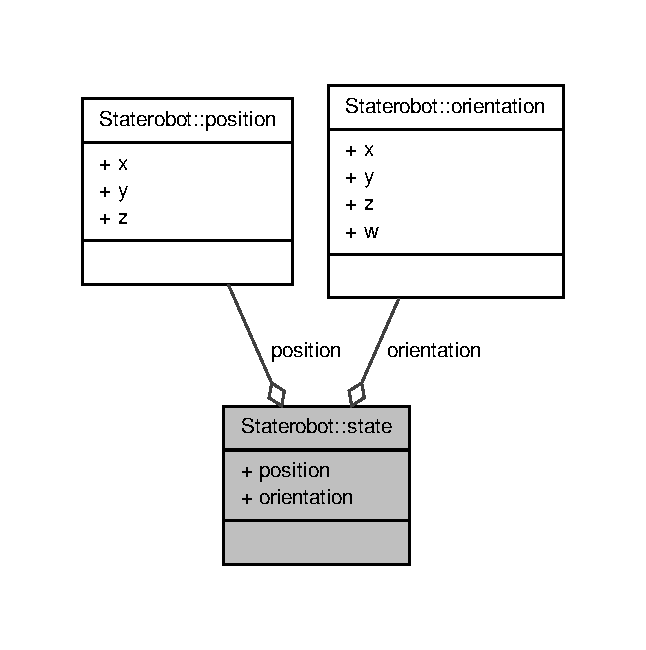
\includegraphics[width=310pt]{struct_staterobot_1_1state__coll__graph}
\end{center}
\end{figure}
\subsection*{\-Public \-Attributes}
\begin{DoxyCompactItemize}
\item 
\hypertarget{struct_staterobot_1_1state_a1b3ab38c820d2a1c70c15d7a52e8e651}{struct \hyperlink{struct_staterobot_1_1position}{position} {\bfseries position}}\label{struct_staterobot_1_1state_a1b3ab38c820d2a1c70c15d7a52e8e651}

\item 
\hypertarget{struct_staterobot_1_1state_a8fee75dc89f771461844a6d39641d163}{struct \hyperlink{struct_staterobot_1_1orientation}{orientation} {\bfseries orientation}}\label{struct_staterobot_1_1state_a8fee75dc89f771461844a6d39641d163}

\end{DoxyCompactItemize}


\-The documentation for this struct was generated from the following file\-:\begin{DoxyCompactItemize}
\item 
include/spiri\-\_\-api/staterobot.\-h\end{DoxyCompactItemize}

\hypertarget{class_staterobot}{\section{Staterobot Class Reference}
\label{class_staterobot}\index{Staterobot@{Staterobot}}
}


Collaboration diagram for Staterobot\-:
\nopagebreak
\begin{figure}[H]
\begin{center}
\leavevmode
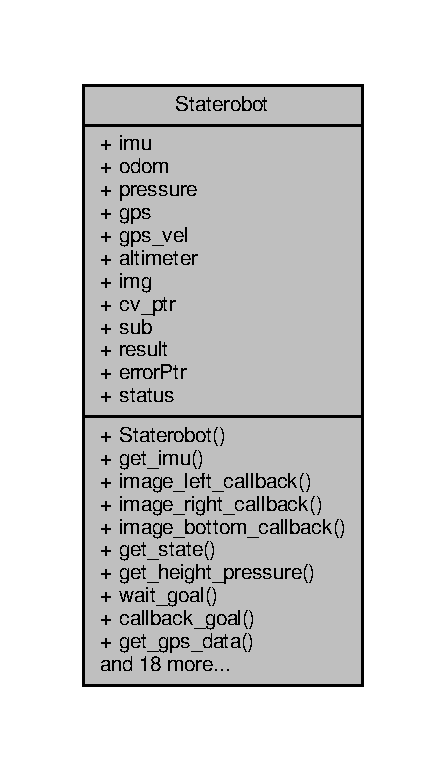
\includegraphics[width=214pt]{class_staterobot__coll__graph}
\end{center}
\end{figure}
\subsection*{Public Member Functions}
\begin{DoxyCompactItemize}
\item 
\hyperlink{class_staterobot_ab99a92f98d724c96989a744aee273155}{Staterobot} ()
\item 
std\-::vector$<$ double $>$ \hyperlink{class_staterobot_a50e002ec81917b295a87463127648a52}{get\-\_\-imu} ()
\item 
\hypertarget{class_staterobot_a4cb41f60186d02b210f354d0199584a4}{void {\bfseries image\-\_\-left\-\_\-callback} (const sensor\-\_\-msgs\-::\-Image\-Const\-Ptr \&)}\label{class_staterobot_a4cb41f60186d02b210f354d0199584a4}

\item 
\hypertarget{class_staterobot_af908b8a70811f3c0a48efe323610602d}{void {\bfseries image\-\_\-right\-\_\-callback} (const sensor\-\_\-msgs\-::\-Image\-Const\-Ptr \&)}\label{class_staterobot_af908b8a70811f3c0a48efe323610602d}

\item 
\hypertarget{class_staterobot_a8ad49fe9f855e5874d8736067fa7fac0}{void {\bfseries image\-\_\-bottom\-\_\-callback} (const sensor\-\_\-msgs\-::\-Image\-Const\-Ptr \&)}\label{class_staterobot_a8ad49fe9f855e5874d8736067fa7fac0}

\item 
std\-::vector$<$ double $>$ \hyperlink{class_staterobot_a51670cc44348eae6328f220421ea328f}{get\-\_\-state} ()
\item 
float \hyperlink{class_staterobot_a0318f7abf24c5c60aee915224af6af02}{get\-\_\-height\-\_\-pressure} ()
\item 
\hypertarget{class_staterobot_a4a44c24dd5cdb773aa40772d02b41720}{bool {\bfseries wait\-\_\-goal} ()}\label{class_staterobot_a4a44c24dd5cdb773aa40772d02b41720}

\item 
\hypertarget{class_staterobot_a37cbdfcb1cc30194f0fa0742952a0aad}{void {\bfseries callback\-\_\-goal} (const action\-\_\-controller\-::\-Multi\-Dof\-Follow\-Joint\-Trajectory\-Action\-Result\-Ptr \&)}\label{class_staterobot_a37cbdfcb1cc30194f0fa0742952a0aad}

\item 
std\-::vector$<$ double $>$ \hyperlink{class_staterobot_a31dcc23cfb620c95e58f3b5ad4bb6b6d}{get\-\_\-gps\-\_\-data} ()
\item 
std\-::vector$<$ double $>$ \hyperlink{class_staterobot_a3a9ee7a49cbb278ffc5f3b201dcae951}{get\-\_\-gps\-\_\-vel} ()
\item 
float \hyperlink{class_staterobot_a3e92b9d6f17c0812e8ed435602d1f717}{get\-\_\-height\-\_\-altimeter} ()
\item 
bool \hyperlink{class_staterobot_a4f1aff1c608a045faa07fa8b9cff4b65}{send\-\_\-goal} (float x, float y, float z, bool relative)
\item 
cv\-::\-Mat \hyperlink{class_staterobot_a5b0323154aa0a19ed82b02cfe7376974}{get\-\_\-left\-\_\-image} ()
\item 
cv\-::\-Mat \hyperlink{class_staterobot_ab1d8f9bfdbd766b96110c0a65fe08f43}{get\-\_\-right\-\_\-image} ()
\item 
cv\-::\-Mat \hyperlink{class_staterobot_a310b2c9315316f96054357ebb705438f}{get\-\_\-bottom\-\_\-image} ()
\item 
void \hyperlink{class_staterobot_a1da31a1c7a8f39878d2511ca86adeb8f}{save\-\_\-image} (const std\-::string, const std\-::string)
\item 
void \hyperlink{class_staterobot_addfc245d53239eed664812a50a916428}{send\-\_\-vel} (float x, float y, float z)
\item 
boost\-::python\-::list \hyperlink{class_staterobot_a3e6bd1883c62204de398342cf8004351}{get\-\_\-imu\-\_\-python} ()
\item 
boost\-::python\-::list \hyperlink{class_staterobot_a91206b2bef7c39193df2eef7b8bae523}{get\-\_\-state\-\_\-python} ()
\item 
boost\-::python\-::list \hyperlink{class_staterobot_ac2fe6ca526d21c1bcb2e284f000759a4}{get\-\_\-gps\-\_\-data\-\_\-python} ()
\item 
boost\-::python\-::list \hyperlink{class_staterobot_aed3a2e6aa076fe6e38f97eb9ab9ef41a}{get\-\_\-gps\-\_\-vel\-\_\-python} ()
\item 
std\-::string \hyperlink{class_staterobot_ab7e02e341f1f3ccfaaa322a2fc1e2caf}{get\-\_\-left\-\_\-image\-\_\-python} ()
\item 
std\-::string \hyperlink{class_staterobot_ab222942f5fe07919fc4999eb600706d1}{get\-\_\-right\-\_\-image\-\_\-python} ()
\item 
std\-::string \hyperlink{class_staterobot_a36d188439ca66b3e56cff58877297945}{get\-\_\-bottom\-\_\-image\-\_\-python} ()
\item 
bool \hyperlink{class_staterobot_abc938e713a748e1803a304e30145e3d1}{send\-\_\-goal\-\_\-python} (boost\-::python\-::list \&)
\item 
bool \hyperlink{class_staterobot_a5ec7a1fdfa9757ddea8c1587e8324f4a}{send\-\_\-goal\-\_\-python\-\_\-relative} (boost\-::python\-::list \&)
\item 
void \hyperlink{class_staterobot_ae47718241f57b27cf4854730cfb50201}{send\-\_\-vel\-\_\-python} (boost\-::python\-::list \&)
\end{DoxyCompactItemize}
\subsection*{Public Attributes}
\begin{DoxyCompactItemize}
\item 
\hypertarget{class_staterobot_ae6075d8fe1f2714e62f98ecfcfabab5f}{sensor\-\_\-msgs\-::\-Imu\-Const\-Ptr {\bfseries imu}}\label{class_staterobot_ae6075d8fe1f2714e62f98ecfcfabab5f}

\item 
\hypertarget{class_staterobot_a647d9af50a8896f64fa9456b5719157b}{nav\-\_\-msgs\-::\-Odometry\-Const\-Ptr {\bfseries odom}}\label{class_staterobot_a647d9af50a8896f64fa9456b5719157b}

\item 
\hypertarget{class_staterobot_a8ab2546d67712dbed7d288f66430d923}{geometry\-\_\-msgs\-::\-Point\-Stamped\-Const\-Ptr {\bfseries pressure}}\label{class_staterobot_a8ab2546d67712dbed7d288f66430d923}

\item 
\hypertarget{class_staterobot_aaade9f6f0d32fb6baaef1c745fa138de}{sensor\-\_\-msgs\-::\-Nav\-Sat\-Fix\-Const\-Ptr {\bfseries gps}}\label{class_staterobot_aaade9f6f0d32fb6baaef1c745fa138de}

\item 
\hypertarget{class_staterobot_a78d4a58c9335c40740c830f7d8499c75}{geometry\-\_\-msgs\-::\-Vector3\-Stamped\-Const\-Ptr {\bfseries gps\-\_\-vel}}\label{class_staterobot_a78d4a58c9335c40740c830f7d8499c75}

\item 
\hypertarget{class_staterobot_a08857351f3bb69c9590778240fcf2d78}{hector\-\_\-uav\-\_\-msgs\-::\-Altimeter\-Const\-Ptr {\bfseries altimeter}}\label{class_staterobot_a08857351f3bb69c9590778240fcf2d78}

\item 
\hypertarget{class_staterobot_abf4b6be91bd0f6be3a78ca438dc38ac2}{sensor\-\_\-msgs\-::\-Image\-Const\-Ptr {\bfseries img}}\label{class_staterobot_abf4b6be91bd0f6be3a78ca438dc38ac2}

\item 
\hypertarget{class_staterobot_aed9668b08e6c38c4008daa836fa88269}{cv\-\_\-bridge\-::\-Cv\-Image\-Ptr {\bfseries cv\-\_\-ptr}}\label{class_staterobot_aed9668b08e6c38c4008daa836fa88269}

\item 
\hypertarget{class_staterobot_a56690a2dc306e9147b373ac8f7145ffa}{image\-\_\-transport\-::\-Subscriber {\bfseries sub}}\label{class_staterobot_a56690a2dc306e9147b373ac8f7145ffa}

\item 
\hypertarget{class_staterobot_a87ce5439fd3c0f2b07a021469819ac43}{action\-\_\-controller\-::\-Multi\-Dof\-Follow\-Joint\-Trajectory\-Action\-Result {\bfseries result}}\label{class_staterobot_a87ce5439fd3c0f2b07a021469819ac43}

\item 
\hypertarget{class_staterobot_aead4ba8f811be3fb0973fc79f7ea7460}{boost\-::shared\-\_\-ptr\\*
$<$ action\-\_\-controller\-::\-Multi\-Dof\-Follow\-Joint\-Trajectory\-Action\-Result \\*
const  $>$ {\bfseries error\-Ptr}}\label{class_staterobot_aead4ba8f811be3fb0973fc79f7ea7460}

\item 
\hypertarget{class_staterobot_a20c4be7ebe29b4995af9d0d498cc063f}{bool {\bfseries status}}\label{class_staterobot_a20c4be7ebe29b4995af9d0d498cc063f}

\end{DoxyCompactItemize}


\subsection{Constructor \& Destructor Documentation}
\hypertarget{class_staterobot_ab99a92f98d724c96989a744aee273155}{\index{Staterobot@{Staterobot}!Staterobot@{Staterobot}}
\index{Staterobot@{Staterobot}!Staterobot@{Staterobot}}
\subsubsection[{Staterobot}]{\setlength{\rightskip}{0pt plus 5cm}Staterobot\-::\-Staterobot (
\begin{DoxyParamCaption}
{}
\end{DoxyParamCaption}
)}}\label{class_staterobot_ab99a92f98d724c96989a744aee273155}
Constructor 

\subsection{Member Function Documentation}
\hypertarget{class_staterobot_a310b2c9315316f96054357ebb705438f}{\index{Staterobot@{Staterobot}!get\-\_\-bottom\-\_\-image@{get\-\_\-bottom\-\_\-image}}
\index{get\-\_\-bottom\-\_\-image@{get\-\_\-bottom\-\_\-image}!Staterobot@{Staterobot}}
\subsubsection[{get\-\_\-bottom\-\_\-image}]{\setlength{\rightskip}{0pt plus 5cm}cv\-::\-Mat Staterobot\-::get\-\_\-bottom\-\_\-image (
\begin{DoxyParamCaption}
{}
\end{DoxyParamCaption}
)}}\label{class_staterobot_a310b2c9315316f96054357ebb705438f}
Get the image from bottom camera

\begin{DoxyReturn}{Returns}
Image (640\-X480) 
\end{DoxyReturn}
\hypertarget{class_staterobot_a36d188439ca66b3e56cff58877297945}{\index{Staterobot@{Staterobot}!get\-\_\-bottom\-\_\-image\-\_\-python@{get\-\_\-bottom\-\_\-image\-\_\-python}}
\index{get\-\_\-bottom\-\_\-image\-\_\-python@{get\-\_\-bottom\-\_\-image\-\_\-python}!Staterobot@{Staterobot}}
\subsubsection[{get\-\_\-bottom\-\_\-image\-\_\-python}]{\setlength{\rightskip}{0pt plus 5cm}std\-::string Staterobot\-::get\-\_\-bottom\-\_\-image\-\_\-python (
\begin{DoxyParamCaption}
{}
\end{DoxyParamCaption}
)}}\label{class_staterobot_a36d188439ca66b3e56cff58877297945}
Get image from the bottom camera

\begin{DoxyReturn}{Returns}
Image which is converted by the python api into a numpy array 
\end{DoxyReturn}
\hypertarget{class_staterobot_a31dcc23cfb620c95e58f3b5ad4bb6b6d}{\index{Staterobot@{Staterobot}!get\-\_\-gps\-\_\-data@{get\-\_\-gps\-\_\-data}}
\index{get\-\_\-gps\-\_\-data@{get\-\_\-gps\-\_\-data}!Staterobot@{Staterobot}}
\subsubsection[{get\-\_\-gps\-\_\-data}]{\setlength{\rightskip}{0pt plus 5cm}std\-::vector$<$ double $>$ Staterobot\-::get\-\_\-gps\-\_\-data (
\begin{DoxyParamCaption}
{}
\end{DoxyParamCaption}
)}}\label{class_staterobot_a31dcc23cfb620c95e58f3b5ad4bb6b6d}
Get the gps position

\begin{DoxyReturn}{Returns}
G\-P\-S (latitude,longitude,altitude) of Spiri 
\end{DoxyReturn}
\hypertarget{class_staterobot_ac2fe6ca526d21c1bcb2e284f000759a4}{\index{Staterobot@{Staterobot}!get\-\_\-gps\-\_\-data\-\_\-python@{get\-\_\-gps\-\_\-data\-\_\-python}}
\index{get\-\_\-gps\-\_\-data\-\_\-python@{get\-\_\-gps\-\_\-data\-\_\-python}!Staterobot@{Staterobot}}
\subsubsection[{get\-\_\-gps\-\_\-data\-\_\-python}]{\setlength{\rightskip}{0pt plus 5cm}boost\-::python\-::list Staterobot\-::get\-\_\-gps\-\_\-data\-\_\-python (
\begin{DoxyParamCaption}
{}
\end{DoxyParamCaption}
)}}\label{class_staterobot_ac2fe6ca526d21c1bcb2e284f000759a4}
Get the gps data

\begin{DoxyReturn}{Returns}
Latitude, longitude and altitude 
\end{DoxyReturn}
\hypertarget{class_staterobot_a3a9ee7a49cbb278ffc5f3b201dcae951}{\index{Staterobot@{Staterobot}!get\-\_\-gps\-\_\-vel@{get\-\_\-gps\-\_\-vel}}
\index{get\-\_\-gps\-\_\-vel@{get\-\_\-gps\-\_\-vel}!Staterobot@{Staterobot}}
\subsubsection[{get\-\_\-gps\-\_\-vel}]{\setlength{\rightskip}{0pt plus 5cm}std\-::vector$<$ double $>$ Staterobot\-::get\-\_\-gps\-\_\-vel (
\begin{DoxyParamCaption}
{}
\end{DoxyParamCaption}
)}}\label{class_staterobot_a3a9ee7a49cbb278ffc5f3b201dcae951}
Get the velocity reporetd by the G\-P\-S

\begin{DoxyReturn}{Returns}
Velocity (x,y,z) of Spiri 
\end{DoxyReturn}
\hypertarget{class_staterobot_aed3a2e6aa076fe6e38f97eb9ab9ef41a}{\index{Staterobot@{Staterobot}!get\-\_\-gps\-\_\-vel\-\_\-python@{get\-\_\-gps\-\_\-vel\-\_\-python}}
\index{get\-\_\-gps\-\_\-vel\-\_\-python@{get\-\_\-gps\-\_\-vel\-\_\-python}!Staterobot@{Staterobot}}
\subsubsection[{get\-\_\-gps\-\_\-vel\-\_\-python}]{\setlength{\rightskip}{0pt plus 5cm}boost\-::python\-::list Staterobot\-::get\-\_\-gps\-\_\-vel\-\_\-python (
\begin{DoxyParamCaption}
{}
\end{DoxyParamCaption}
)}}\label{class_staterobot_aed3a2e6aa076fe6e38f97eb9ab9ef41a}
Velocity reported by G\-P\-S

\begin{DoxyReturn}{Returns}
Velocity in x,y and z direction 
\end{DoxyReturn}
\hypertarget{class_staterobot_a3e92b9d6f17c0812e8ed435602d1f717}{\index{Staterobot@{Staterobot}!get\-\_\-height\-\_\-altimeter@{get\-\_\-height\-\_\-altimeter}}
\index{get\-\_\-height\-\_\-altimeter@{get\-\_\-height\-\_\-altimeter}!Staterobot@{Staterobot}}
\subsubsection[{get\-\_\-height\-\_\-altimeter}]{\setlength{\rightskip}{0pt plus 5cm}float Staterobot\-::get\-\_\-height\-\_\-altimeter (
\begin{DoxyParamCaption}
{}
\end{DoxyParamCaption}
)}}\label{class_staterobot_a3e92b9d6f17c0812e8ed435602d1f717}
Get the height in metres from altimeter

\begin{DoxyReturn}{Returns}
Altitude of Spiri 
\end{DoxyReturn}
\hypertarget{class_staterobot_a0318f7abf24c5c60aee915224af6af02}{\index{Staterobot@{Staterobot}!get\-\_\-height\-\_\-pressure@{get\-\_\-height\-\_\-pressure}}
\index{get\-\_\-height\-\_\-pressure@{get\-\_\-height\-\_\-pressure}!Staterobot@{Staterobot}}
\subsubsection[{get\-\_\-height\-\_\-pressure}]{\setlength{\rightskip}{0pt plus 5cm}float Staterobot\-::get\-\_\-height\-\_\-pressure (
\begin{DoxyParamCaption}
{}
\end{DoxyParamCaption}
)}}\label{class_staterobot_a0318f7abf24c5c60aee915224af6af02}
Get the height in metres from pressure sensor

\begin{DoxyReturn}{Returns}
Altitude of Spiri 
\end{DoxyReturn}
\hypertarget{class_staterobot_a50e002ec81917b295a87463127648a52}{\index{Staterobot@{Staterobot}!get\-\_\-imu@{get\-\_\-imu}}
\index{get\-\_\-imu@{get\-\_\-imu}!Staterobot@{Staterobot}}
\subsubsection[{get\-\_\-imu}]{\setlength{\rightskip}{0pt plus 5cm}std\-::vector$<$ double $>$ Staterobot\-::get\-\_\-imu (
\begin{DoxyParamCaption}
{}
\end{DoxyParamCaption}
)}}\label{class_staterobot_a50e002ec81917b295a87463127648a52}
Get the orientation in quaternion from I\-M\-U

\begin{DoxyReturn}{Returns}
Orientation (x,y,z,w) of Spiri 
\end{DoxyReturn}
\hypertarget{class_staterobot_a3e6bd1883c62204de398342cf8004351}{\index{Staterobot@{Staterobot}!get\-\_\-imu\-\_\-python@{get\-\_\-imu\-\_\-python}}
\index{get\-\_\-imu\-\_\-python@{get\-\_\-imu\-\_\-python}!Staterobot@{Staterobot}}
\subsubsection[{get\-\_\-imu\-\_\-python}]{\setlength{\rightskip}{0pt plus 5cm}boost\-::python\-::list Staterobot\-::get\-\_\-imu\-\_\-python (
\begin{DoxyParamCaption}
{}
\end{DoxyParamCaption}
)}}\label{class_staterobot_a3e6bd1883c62204de398342cf8004351}
Get orientation from I\-M\-U

\begin{DoxyReturn}{Returns}
The orientation in quaternion (x,y,z,w) 
\end{DoxyReturn}
\hypertarget{class_staterobot_a5b0323154aa0a19ed82b02cfe7376974}{\index{Staterobot@{Staterobot}!get\-\_\-left\-\_\-image@{get\-\_\-left\-\_\-image}}
\index{get\-\_\-left\-\_\-image@{get\-\_\-left\-\_\-image}!Staterobot@{Staterobot}}
\subsubsection[{get\-\_\-left\-\_\-image}]{\setlength{\rightskip}{0pt plus 5cm}cv\-::\-Mat Staterobot\-::get\-\_\-left\-\_\-image (
\begin{DoxyParamCaption}
{}
\end{DoxyParamCaption}
)}}\label{class_staterobot_a5b0323154aa0a19ed82b02cfe7376974}
Get the image from left front camera.

\begin{DoxyReturn}{Returns}
Image (640\-X480) 
\end{DoxyReturn}
\hypertarget{class_staterobot_ab7e02e341f1f3ccfaaa322a2fc1e2caf}{\index{Staterobot@{Staterobot}!get\-\_\-left\-\_\-image\-\_\-python@{get\-\_\-left\-\_\-image\-\_\-python}}
\index{get\-\_\-left\-\_\-image\-\_\-python@{get\-\_\-left\-\_\-image\-\_\-python}!Staterobot@{Staterobot}}
\subsubsection[{get\-\_\-left\-\_\-image\-\_\-python}]{\setlength{\rightskip}{0pt plus 5cm}std\-::string Staterobot\-::get\-\_\-left\-\_\-image\-\_\-python (
\begin{DoxyParamCaption}
{}
\end{DoxyParamCaption}
)}}\label{class_staterobot_ab7e02e341f1f3ccfaaa322a2fc1e2caf}
Get image from the left camera

\begin{DoxyReturn}{Returns}
Image which is converted by the python api into a numpy array 
\end{DoxyReturn}
\hypertarget{class_staterobot_ab1d8f9bfdbd766b96110c0a65fe08f43}{\index{Staterobot@{Staterobot}!get\-\_\-right\-\_\-image@{get\-\_\-right\-\_\-image}}
\index{get\-\_\-right\-\_\-image@{get\-\_\-right\-\_\-image}!Staterobot@{Staterobot}}
\subsubsection[{get\-\_\-right\-\_\-image}]{\setlength{\rightskip}{0pt plus 5cm}cv\-::\-Mat Staterobot\-::get\-\_\-right\-\_\-image (
\begin{DoxyParamCaption}
{}
\end{DoxyParamCaption}
)}}\label{class_staterobot_ab1d8f9bfdbd766b96110c0a65fe08f43}
Get the image from right front camera

\begin{DoxyReturn}{Returns}
Image (640\-X480) 
\end{DoxyReturn}
\hypertarget{class_staterobot_ab222942f5fe07919fc4999eb600706d1}{\index{Staterobot@{Staterobot}!get\-\_\-right\-\_\-image\-\_\-python@{get\-\_\-right\-\_\-image\-\_\-python}}
\index{get\-\_\-right\-\_\-image\-\_\-python@{get\-\_\-right\-\_\-image\-\_\-python}!Staterobot@{Staterobot}}
\subsubsection[{get\-\_\-right\-\_\-image\-\_\-python}]{\setlength{\rightskip}{0pt plus 5cm}std\-::string Staterobot\-::get\-\_\-right\-\_\-image\-\_\-python (
\begin{DoxyParamCaption}
{}
\end{DoxyParamCaption}
)}}\label{class_staterobot_ab222942f5fe07919fc4999eb600706d1}
Get image from the right camera

\begin{DoxyReturn}{Returns}
Image which is converted by the python api into a numpy array 
\end{DoxyReturn}
\hypertarget{class_staterobot_a51670cc44348eae6328f220421ea328f}{\index{Staterobot@{Staterobot}!get\-\_\-state@{get\-\_\-state}}
\index{get\-\_\-state@{get\-\_\-state}!Staterobot@{Staterobot}}
\subsubsection[{get\-\_\-state}]{\setlength{\rightskip}{0pt plus 5cm}std\-::vector$<$ double $>$ Staterobot\-::get\-\_\-state (
\begin{DoxyParamCaption}
{}
\end{DoxyParamCaption}
)}}\label{class_staterobot_a51670cc44348eae6328f220421ea328f}
Get the state

\begin{DoxyReturn}{Returns}
Position(x,y,z) and orientation (x,y,z,w) of Spiri 
\end{DoxyReturn}
\hypertarget{class_staterobot_a91206b2bef7c39193df2eef7b8bae523}{\index{Staterobot@{Staterobot}!get\-\_\-state\-\_\-python@{get\-\_\-state\-\_\-python}}
\index{get\-\_\-state\-\_\-python@{get\-\_\-state\-\_\-python}!Staterobot@{Staterobot}}
\subsubsection[{get\-\_\-state\-\_\-python}]{\setlength{\rightskip}{0pt plus 5cm}boost\-::python\-::list Staterobot\-::get\-\_\-state\-\_\-python (
\begin{DoxyParamCaption}
{}
\end{DoxyParamCaption}
)}}\label{class_staterobot_a91206b2bef7c39193df2eef7b8bae523}
Get the state of Spiri

\begin{DoxyReturn}{Returns}
Position(x,y,z) and orientation(x,y,z,w) 
\end{DoxyReturn}
\hypertarget{class_staterobot_a1da31a1c7a8f39878d2511ca86adeb8f}{\index{Staterobot@{Staterobot}!save\-\_\-image@{save\-\_\-image}}
\index{save\-\_\-image@{save\-\_\-image}!Staterobot@{Staterobot}}
\subsubsection[{save\-\_\-image}]{\setlength{\rightskip}{0pt plus 5cm}void Staterobot\-::save\-\_\-image (
\begin{DoxyParamCaption}
\item[{const std\-::string}]{path = {\ttfamily \char`\"{}\char`\"{}}, }
\item[{const std\-::string}]{camera = {\ttfamily \char`\"{}\char`\"{}}}
\end{DoxyParamCaption}
)}}\label{class_staterobot_a1da31a1c7a8f39878d2511ca86adeb8f}
Save the image


\begin{DoxyParams}{Parameters}
{\em path} & location to save the files \\
\hline
{\em camera} & which camera to save the image from \mbox{[}left,right,bottom\mbox{]}\\
\hline
\end{DoxyParams}
\begin{DoxyReturn}{Returns}
Image (640\-X480) 
\end{DoxyReturn}
\hypertarget{class_staterobot_a4f1aff1c608a045faa07fa8b9cff4b65}{\index{Staterobot@{Staterobot}!send\-\_\-goal@{send\-\_\-goal}}
\index{send\-\_\-goal@{send\-\_\-goal}!Staterobot@{Staterobot}}
\subsubsection[{send\-\_\-goal}]{\setlength{\rightskip}{0pt plus 5cm}bool Staterobot\-::send\-\_\-goal (
\begin{DoxyParamCaption}
\item[{float}]{x, }
\item[{float}]{y, }
\item[{float}]{z, }
\item[{bool}]{relative = {\ttfamily false}}
\end{DoxyParamCaption}
)}}\label{class_staterobot_a4f1aff1c608a045faa07fa8b9cff4b65}
Send goal to Spiri


\begin{DoxyParams}{Parameters}
{\em x} & coordinate in x direction \\
\hline
{\em y} & coordinate in y direction \\
\hline
{\em z} & coordinate in z direction \\
\hline
{\em relative} & If set then goal is calculated with respect to the start position otherwise coordinates are with respect to the world\\
\hline
\end{DoxyParams}
\begin{DoxyReturn}{Returns}
Succesfully executed or not 
\end{DoxyReturn}
\hypertarget{class_staterobot_abc938e713a748e1803a304e30145e3d1}{\index{Staterobot@{Staterobot}!send\-\_\-goal\-\_\-python@{send\-\_\-goal\-\_\-python}}
\index{send\-\_\-goal\-\_\-python@{send\-\_\-goal\-\_\-python}!Staterobot@{Staterobot}}
\subsubsection[{send\-\_\-goal\-\_\-python}]{\setlength{\rightskip}{0pt plus 5cm}bool Staterobot\-::send\-\_\-goal\-\_\-python (
\begin{DoxyParamCaption}
\item[{boost\-::python\-::list \&}]{values}
\end{DoxyParamCaption}
)}}\label{class_staterobot_abc938e713a748e1803a304e30145e3d1}
Send goal to Spiri with respect to the world


\begin{DoxyParams}{Parameters}
{\em values} & Cooridinates in x,y,z\\
\hline
\end{DoxyParams}
\begin{DoxyReturn}{Returns}
Succesfull 
\end{DoxyReturn}
\hypertarget{class_staterobot_a5ec7a1fdfa9757ddea8c1587e8324f4a}{\index{Staterobot@{Staterobot}!send\-\_\-goal\-\_\-python\-\_\-relative@{send\-\_\-goal\-\_\-python\-\_\-relative}}
\index{send\-\_\-goal\-\_\-python\-\_\-relative@{send\-\_\-goal\-\_\-python\-\_\-relative}!Staterobot@{Staterobot}}
\subsubsection[{send\-\_\-goal\-\_\-python\-\_\-relative}]{\setlength{\rightskip}{0pt plus 5cm}bool Staterobot\-::send\-\_\-goal\-\_\-python\-\_\-relative (
\begin{DoxyParamCaption}
\item[{boost\-::python\-::list \&}]{values}
\end{DoxyParamCaption}
)}}\label{class_staterobot_a5ec7a1fdfa9757ddea8c1587e8324f4a}
Send goal to Spiri with respect to the current position


\begin{DoxyParams}{Parameters}
{\em values} & Cooridinates in x,y,z\\
\hline
\end{DoxyParams}
\begin{DoxyReturn}{Returns}
Succesfull 
\end{DoxyReturn}
\hypertarget{class_staterobot_addfc245d53239eed664812a50a916428}{\index{Staterobot@{Staterobot}!send\-\_\-vel@{send\-\_\-vel}}
\index{send\-\_\-vel@{send\-\_\-vel}!Staterobot@{Staterobot}}
\subsubsection[{send\-\_\-vel}]{\setlength{\rightskip}{0pt plus 5cm}void Staterobot\-::send\-\_\-vel (
\begin{DoxyParamCaption}
\item[{float}]{x, }
\item[{float}]{y, }
\item[{float}]{z}
\end{DoxyParamCaption}
)}}\label{class_staterobot_addfc245d53239eed664812a50a916428}
Send velocity to Spiri.


\begin{DoxyParams}{Parameters}
{\em x} & velocity in x direction \\
\hline
{\em y} & velocity in y direction \\
\hline
{\em z} & velocity in z direction \\
\hline
\end{DoxyParams}
\begin{DoxyRefDesc}{Todo}
\item[\hyperlink{todo__todo000004}{Todo}]This is hack. If there exists a better way in R\-O\-S need to find that \end{DoxyRefDesc}
\hypertarget{class_staterobot_ae47718241f57b27cf4854730cfb50201}{\index{Staterobot@{Staterobot}!send\-\_\-vel\-\_\-python@{send\-\_\-vel\-\_\-python}}
\index{send\-\_\-vel\-\_\-python@{send\-\_\-vel\-\_\-python}!Staterobot@{Staterobot}}
\subsubsection[{send\-\_\-vel\-\_\-python}]{\setlength{\rightskip}{0pt plus 5cm}void Staterobot\-::send\-\_\-vel\-\_\-python (
\begin{DoxyParamCaption}
\item[{boost\-::python\-::list \&}]{val}
\end{DoxyParamCaption}
)}}\label{class_staterobot_ae47718241f57b27cf4854730cfb50201}
Send velocity commands to Spiri


\begin{DoxyParams}{Parameters}
{\em val} & Velocities in m/s in x,y,z direction \\
\hline
\end{DoxyParams}


The documentation for this class was generated from the following files\-:\begin{DoxyCompactItemize}
\item 
include/spiri\-\_\-api/staterobot.\-h\item 
src/staterobot.\-cpp\end{DoxyCompactItemize}

\printindex
\end{document}
